% ОБЯЗАТЕЛЬНО ИМЕННО ТАКОЙ documentclass!
% (Основной кегль = 14pt, поэтому необходим "extsizes")
% Формат, разумеется, А4
% article потому что стандарт не подразумевает разделов
% Глава = section, Параграф = subsection
% (понятия "глава" и "параграф" из стандарта)
\documentclass[a4paper,article,14pt]{extarticle}

% Подключаем главный пакет со всем необходимым
\usepackage{spbudiploma_tempora}
% Пакеты по желанию (самые распространенные)
% Хитрые мат. символы
\usepackage{euscript}
% Таблицы
\usepackage{longtable}
\usepackage{makecell}
% Картинки (можно вставлять даже pdf)
\usepackage[pdftex]{graphicx}

\usepackage{amsthm,amssymb, amsmath}
\usepackage{textcomp}
\usepackage{pdfpages}

\begin{document}

% Титульный лист в файле titlepage.tex

\includepdf[page=-]{images/tit.pdf}
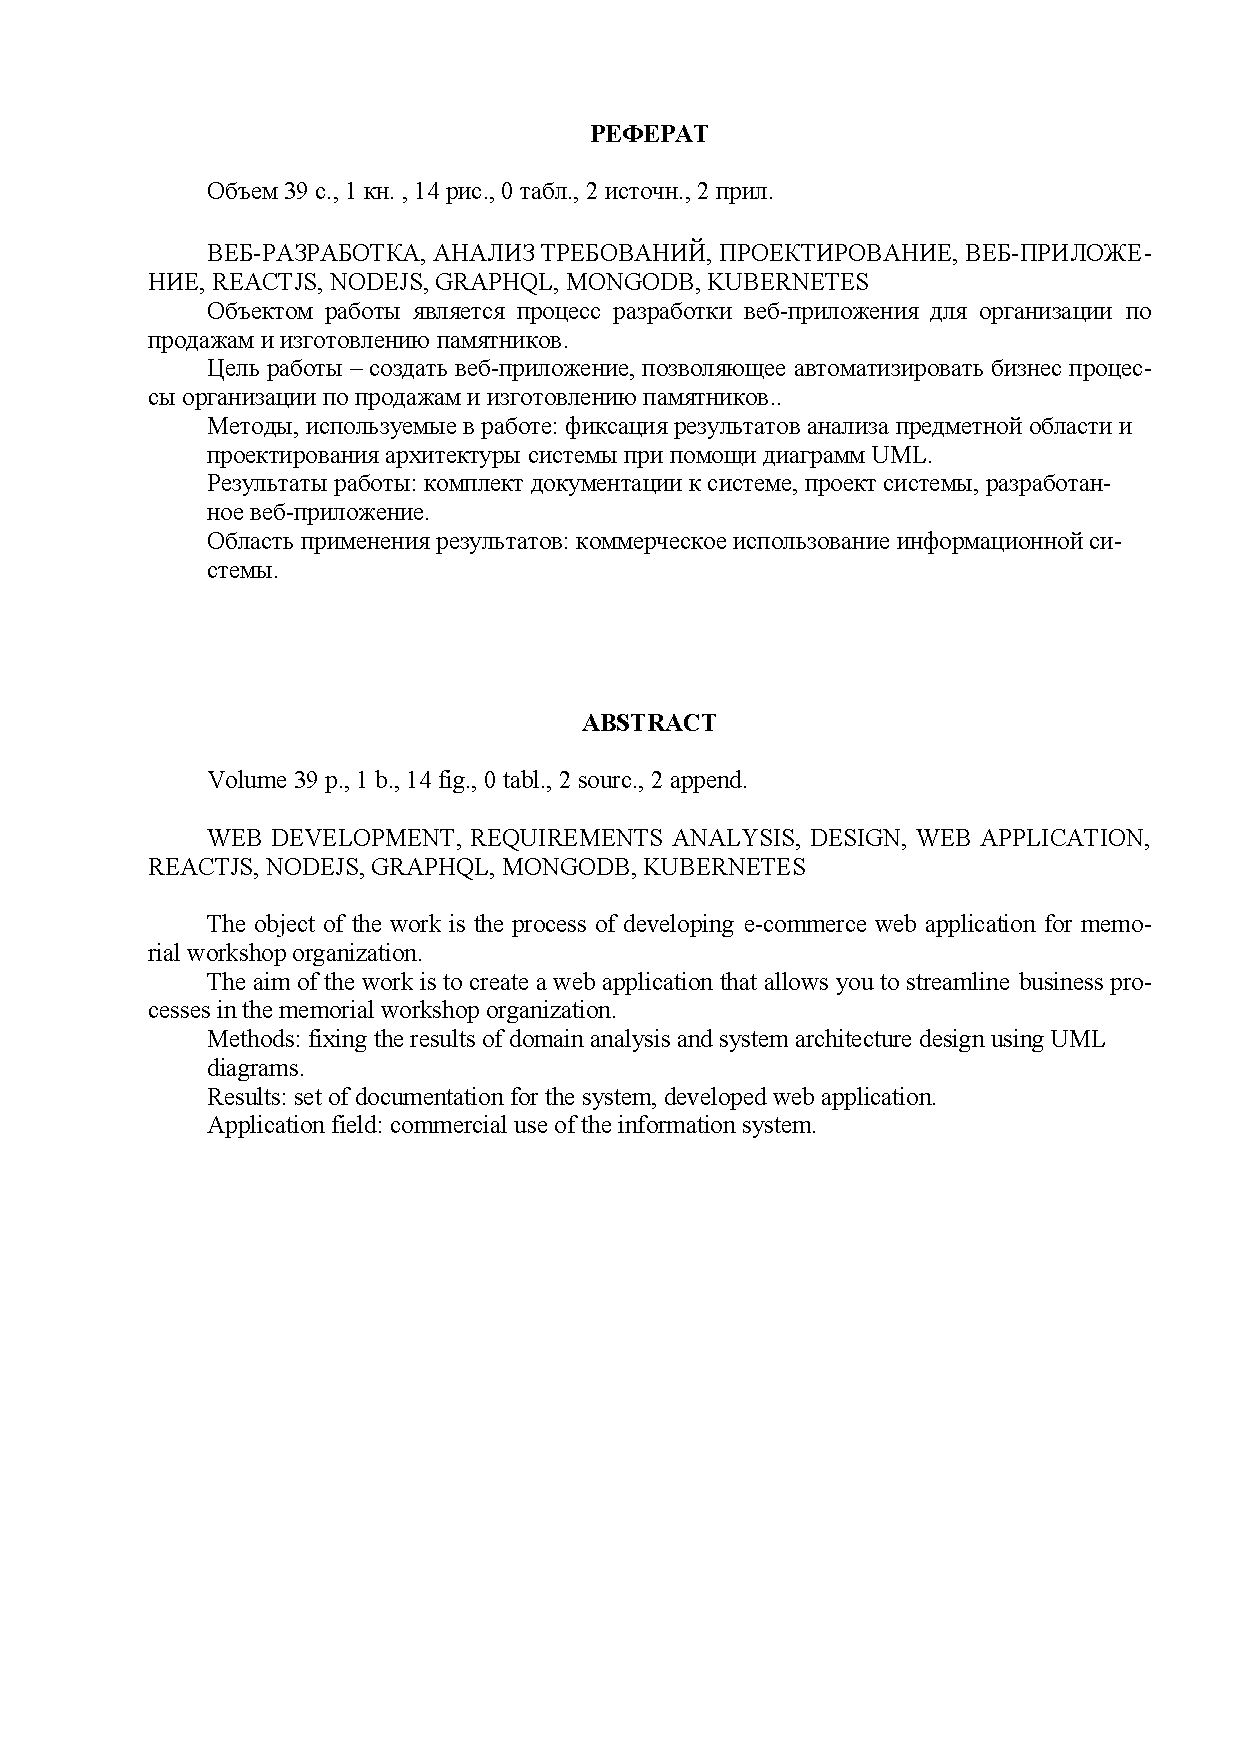
\includepdf[page=-]{images/abs.pdf}

\specialsection{Определения, обозначения сокращения}
БД - База данных
ОС - Операционная система
ПО - Программное обеспечение
СУБД - Система управления базами данных
POC - proof of concept
ЯП - язык программирования
REST - Representational state transfer
SPA - Single page application
k8s - Kubernetes

\pagebreak

% Содержание
\tableofcontents
\pagebreak


\includepdf[page=-]{images/zad.pdf}


\includepdf[page=-]{images/cal.pdf}




\specialsection{Введение}

Одной из наиболее активно развивающихся отраслей в нашей стране является отрасль ритуальных услуг,
в том числе изготовление ритуальных памятников. 
В данной сфере до сих пор нет четко выраженного лидера, велика доля малого бизнеса.
Гораздо чаще люди обращаются за услугой оффлайн.

Внедрение цифровых технологий как никогда актуально в этой отрасли из-за пандемии COVID-19.
В России, как и во всем мире, выросла смертность, с этим нетрудно связать увеличение числа клиентов и заказов в сфере ритуальных услуг.
Памятник обычно ставят через год после погребения усопшего, а пандемия началась ровно год назад,
это значит что в этом году ожидается резкий подъем продаж. 
Также из-за карантинов и новых правил самоизоляции какое-то время не могли работать офисы и торговые точки. 
После внедрения цифровых технологий сотрудники организаций этой отрасли смогут работать удаленно, а клиенты получать услугу дистанционно.

Цель данной работы – разработать систему для оформления заказов ритуальных памятников,
которая поможет решить проблемы поставленные заказчиком, которая в то же время будет универсальным и гибким решением, которое может
подходить и другим компаниям в этой сфере.
\pagebreak

\specialsection{Постановка задач}

В рамках разработки приложения необходимо решить множество задач. Основными из которых являются:

\begin{enumerate}
    \item Проанализировать предметную область, проблемы и требования заказчика
    \item Определить основные функциональные возможности и варианты использования системы
    \item Выбрать архитектуру и технологии разработки наиболее подходящие для разработки системы
    \item Спроектировать и сконструировать систему используя знания полученные в ходе анализа
    \item Протестировать и выполнить деплой системы
\end{enumerate}


\section{Разработка и анализ требований}

В этой главе будет рассмотрена предметная область, а также анализированы требования к разрабатываемой системе.
Также будут определены основные варианты использования.

\subsection{Заказчик}
Заказчиком системы является небольшая компания по изготовлению и продаже памятников из гранита. 
Данную компанию можно охарактеризовать как семейный бизнес.
Владельцы бизнеса, также являются и управляющими компанией. 
Тем не менее в этой компании есть некоторое количество наемных рабочих, которые выполняют роль менеджеров по продажам.
Всего у компании есть три точки продаж в одной области.

Следовательно, система будет разрабатываться для конкретного заказчика, значит требования должны учитывать проблемы и желания
конкретного заказчика. Тем не менее, было решено разрабатывать универсальную систему, для небольших салонов по изготовлению
 и продаже памятников.

У заказчика еще нет интернет сайта и магазина так как у него нет проблем с привлечением клиентов оффлайн.

\subsection{Предметная область}

Предметная область смоделирована с помощью Диаграммы классов UML, которая представлена на рисунке \ref{uml1}.

Главной сущностью в предметной области заказа памятников является заказ.
Основная информация в заказе это информация о товарах и клиенте, данные усопшего.
Помимо этого также есть, например, информация о менеджере и отделении ответственных за этот заказ.

Главное отличие заказа в рассматриваемой предметной области от других бизнесов связанных с торговлей является то, что
памятник часто заказывают индивидуально и выбирают каждую часть отдельно:

\begin{itemize}
    \item Памятник состоит из множества частей: стеллы, подставки, цветника, надгробия, и т.д.
    \item Также на памятник наносят индивидуальное оформление, гравировку или фотокерамику
    \item В дополнение к памятнику могут также заказать металлический забор, ворота, столик, скамейку, а так же всевозможные изделия из гранита
    \item К каждому элементу заказа предлагается целый ряд обязательных 
    или опциональных услуг которые зависят как от свойств самого элемента, так и от желания клиента
\end{itemize}

Таким образом, получается огромное число возможных вариантов заказа, в то время как в обычных интернет магазинах у одного
товара как правило есть всего один или несколько вариантов а также есть четкая цена. 
Для типовых недорогих памятников есть готовые комплекты с фиксированными ценами, 
но там уже гораздо меньше возможностей индивидуального оформления.

Каждая часть памятника и каждый элемент заказа описывается в документе ``Наряд-Заказ'', 
также вместе с ним оформляется документ ``Договор'', который фиксирует итоговую цену а также описывает права и обязанности бизнеса и покупателя.

\begin{figure}[ht]
\begin{center}
\scalebox{0.4}{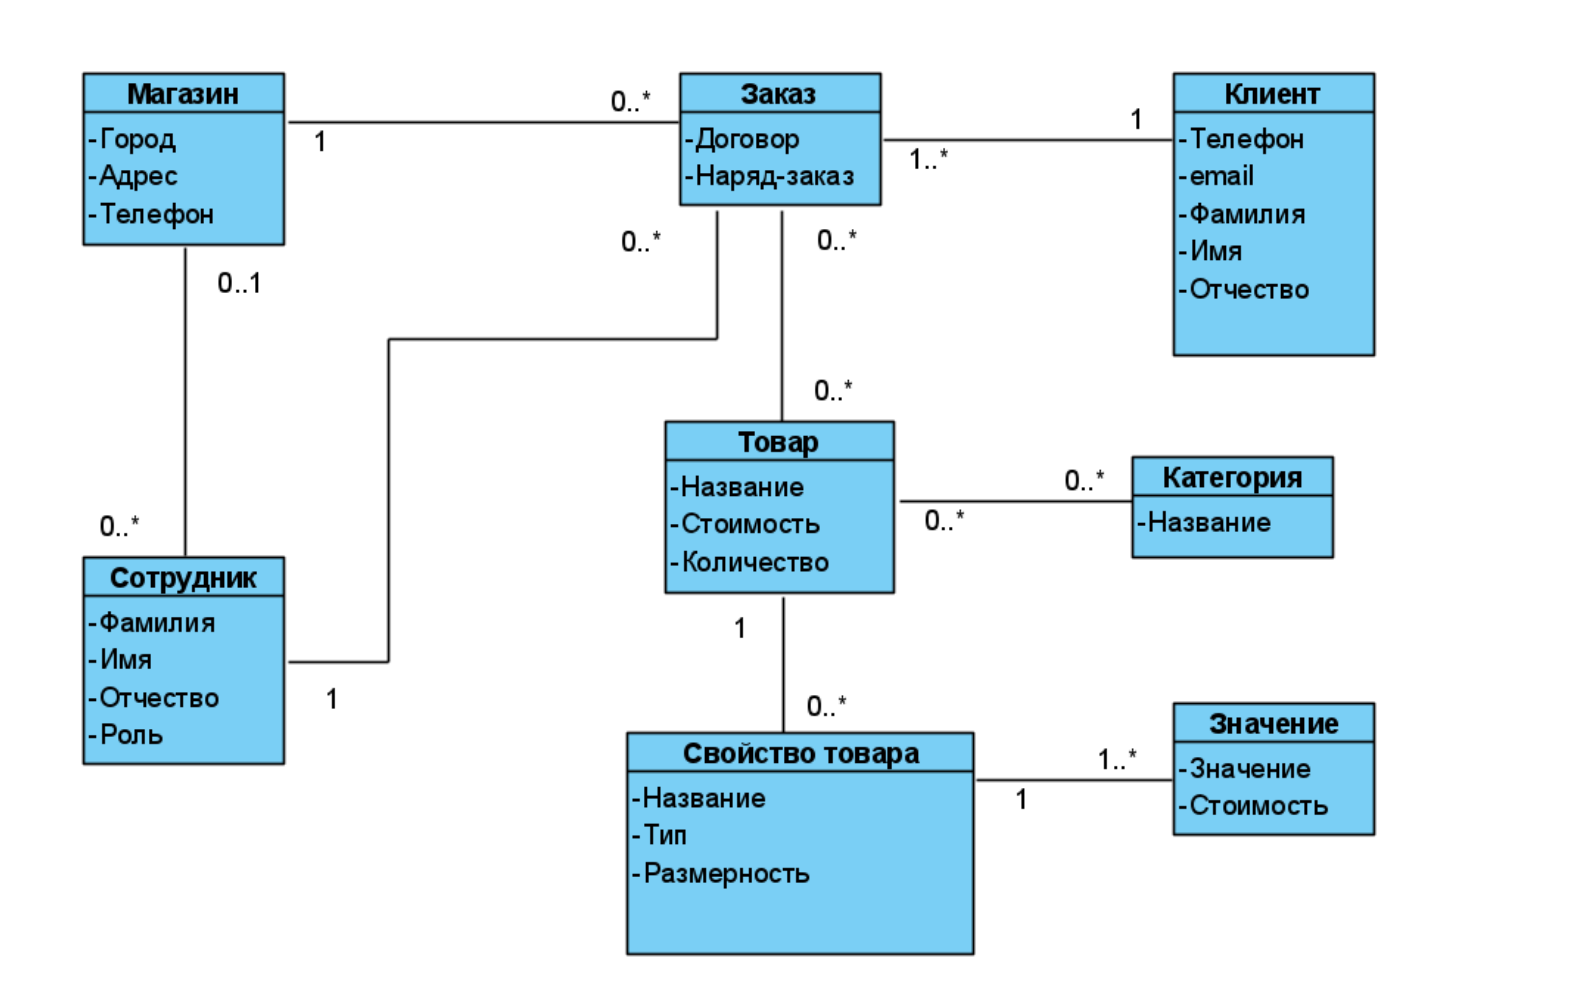
\includegraphics{images/uml1.png}}
\caption{\label{uml1} Диаграмма классов предметной области.}
\end {center}
\end {figure}

\subsection{Основные бизнес правила}

\begin{itemize}
  \item Чтобы совершить заказа, клиент обязан прийти в отделение компании
  \item Клиент может оплатить заказ только наличными или банковским переводом с карты на карту в отдельных случаях
  \item Изготовление стеллы начинается после того как заказ была оплачен
\end{itemize}

\subsection{Проблемы}
\begin{itemize}
    \item Ошибки в заказах, так как они оформляются от руки
    \item Менеджеры по продажам плохо разбираются в вопросах предметной области, 
    например выбирают слишком маленькую подставку для слишком большой стелы
    \item Для управления расценками и каталогом используется простой текстовый документ и описывает только самые типовые модели
    \item Продавцы часто не знают сколько будет стоить изготовить памятник с произвольным, не типовым оформлением
    \item Управляющим сложно следить за всеми заказами и поставками, 
    так как сейчас эта информация передается устно и записывается только в excel таблицу
\end{itemize}

\subsection{Варианты использования}

Основные варианты использования системы описаны с помощью диаграммы вариантов использования в нотации UML.
Диаграмма представлена на рисунке \ref{uml2}:

\begin{enumerate}
    \item Оформление заказа, добавление информации о стелле и об усопшем 
    \item Поиск заказа - по номеру телефона и номеру заказа
    \item Информация о наличии товара на складе и резервирование
    \item Печать документов
\end{enumerate}

\begin{figure}[ht]
\begin{center}
\scalebox{0.4}{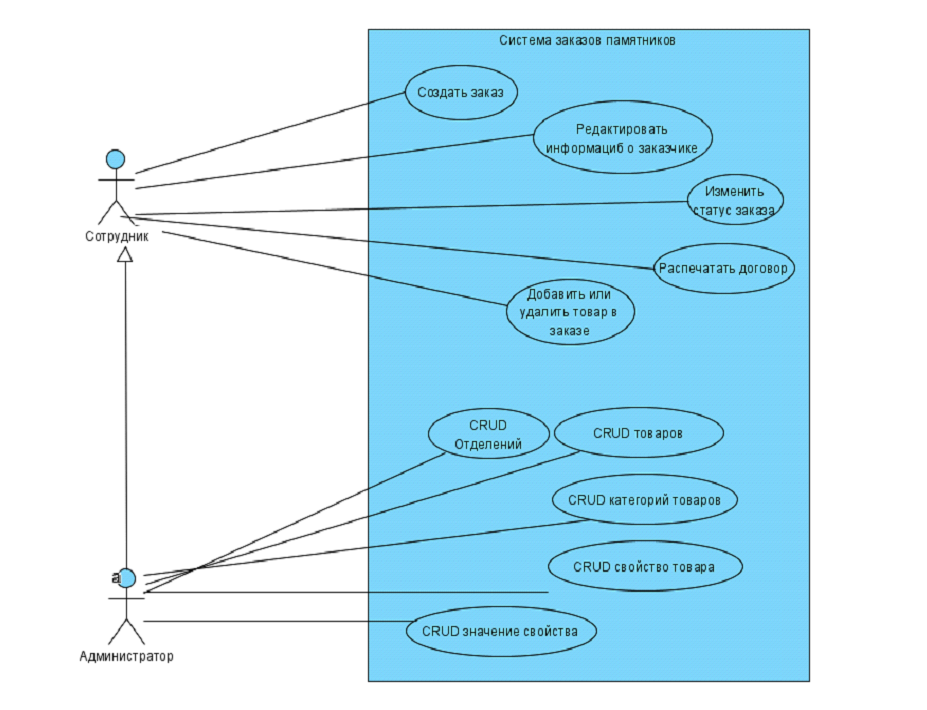
\includegraphics{images/uml2.png}}
\caption{\label{uml2} Диаграмма вариантов использования.}
\end {center}
\end {figure}
    
\subsection{Ограничения}

\begin{itemize}
    \item Поддержка только русского языка, так как у конкретного заказчика есть магазины только в одной области в России.
    Также предметная область специфична для России и стран СНГ.
    \item Заказчик и другие потенциальные клиенты являются представителями малого бизнеса
    Следовательно системой будут пользоваться ограниченное число пользователей, и магазинов в системе будет магазинов не так много.
    Это накладывает ограничение как и на трафик, который будет маленьким, так и на процесс.
    Так как в маленьких магазинах чаще всего нет четкого разделения ролей между продавцами.
    \item В одном заказе может быть только одна стелла. Это ограничение нужно для упрощения логики обработки заказов.
\end{itemize}

\subsection{Постановка целей перед системой}

Основная цель системы – решать проблемы основного заказчика, а именно приложение должно:

\begin{enumerate}
  \item Сократить время необходимое на оформление и обработку заказов на 30\%
  \item Сократить количество ошибок в заказах на 50\%
  \item Сократить время необходимое на обучение сотрудника до 1 недели.
\end{enumerate}
\pagebreak

\section{Проектирование}

В этой главе будут рассмотрены основные проектные решения выполненные при проектировании и разработки системы для заказа памятников.
При выборе технологии, я руководствовался в основном тремя факторами:

\begin{enumerate}
    \item популярность и размер сообщества;
    \item гибкость и масштабируемость;
    \item открытая код и лицензия.
\end{enumerate}

При проектировании я пытался сделать систему как можно более гибкой.

\subsection{Выбор платформы}

Основным пользователем приложения являются сотрудники бизнеса, 
основным устройством которых являются либо моноблок, либо ноутбук.

Таким образом следует разрабатывать либо настольное приложение, либо веб-приложение.

В качестве платформы для разработки был выбран веб, на это имеется две основные причины:

\begin{enumerate}
    \item Стоимость разработки гораздо ниже чем у desktop приложений. Это обусловлено развитием сообщества библиотек, фреймворков, 
    инструментов и приложений с открытым исходным кодом, 
    а именно наличием большого количества готовых компонентов для решения типовых задач бизнес.
    \item Универсальность, почти все платформы поддерживают веб, так что приложение не привязано к ОС.
    Так что в теории заказчик может отказаться от ОС MS Windows и перейти на linux чтобы сократить издержки.
\end{enumerate}
\pagebreak

\subsection{Выбор архитектуры приложения}

Приложение будет иметь традиционную монолитную трехслойную архитектуру и будет использовать технологии стека MERNG: MongoDB, Express,
ReactJS, NodeJS, GraphQL. Слои перечислены ниже:

\begin{enumerate}
    \item Слой данных - сервер баз данных MongoDB
    \item Слой API - сервер express-graphql-apollo
    \item Слой представления - SPA ReactJS клиент
\end{enumerate}

Монолитная архитектуру была выбрана в первую очередь из-за ограниченности ресурсов. 
Микросервисная архитектуру в первую очередь нужна когда проект слишком большой,
и его проще разбить на отдельные сервисы, с целью распараллелить разработку на несколько команд разработчиков.

Также микросервисная архитектура упрощает поддержку и увеличивает гибкость при деплое приложения.

Но так как разрабатывать приложение для заказа памятников будет только один человек, использовать микросервисную архитектуру особого смысла не имеет.

\subsection{Выбор языка программирования}

Основным языком программирования в вебе является JavaScript, а также TypeScript. 
Также сейчас развивается WebAssembly, он позволяет компилировать почти любой ЯП в низкоуровневый код который понимает браузер.
В теории это позволяет писать приложения который быстрее работают и загружаются. Однако прирост производительности тут не очень велик, 
по сравнению с увеличением стоимости разработки. Поэтому выбор был сделан в пользу TypeScript.

\subsection{Выбор технологий backend}

В качестве протокола был выбран GraphQL в первую очередь из-за его популярности а также желания,
его изучить, и освоить навыки разработки приложений с его применением. Также он неплохо подходит для приложения.

Основные преимущества GraphQL:

\begin{itemize}
    \item возможность писать гибкие запросы и получать только те данные которые нужны
    \item встроенная проверка типов времени выполнения
\end{itemize}

Однако у GraphQL протокола есть главные недостаток, он заставляет проектировать схему запросов.
Проектирование которой требует хорошего знания предметной области и GraphQL [1]. 

Также кроме этого традиционные REST протоколы выигрывают в производительности в несколько раз, за счет того что 
GraphQL вносит много своих издержек производительности, а также его сложнее кешировать на уровне API. 

Однако вопросы производительности GraphQL выходят за рамки поставленных ограничений.

Помимо основного backend, в приложении также есть дополнительный backend для потенциального интернет магазина клиента.
Прямо сейчас у заказчика нет своего интернет магазина, но для того чтобы расширить гибкость и функционал системы было принято решение
добавить REST endpoint, а также в рамках работы создать POC клиента интернет магазина.

Диаграмма архитектуры представлена на рисунке \ref{arch}

\begin{figure}[ht]
\begin{center}
\scalebox{0.55}{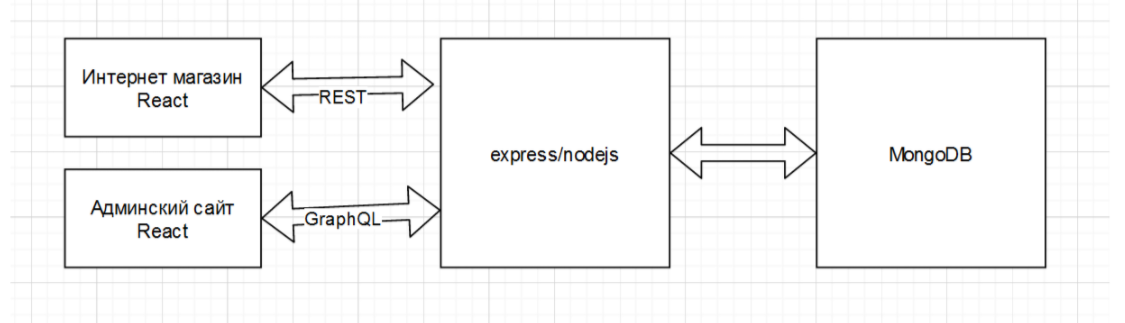
\includegraphics{images/arch.png}}
\caption{\label{arch} Диаграмма сущностей базы данных относящихся к функционалу создания заказа}
\end {center}
\end {figure}

\subsection{Выбор технологий frontend}

В качестве клиента выступает SPA endpoint. Для разработки SPA будет использоваться библиотека ReactJS.
А также фреймворк Apollo Client React. 
В качестве набора компонентов будет использоваться отдельная библиотека разработанная в рамках данной ВКР специально для
этого приложения. Но данная библиотека спроектирована универсально для любых приложений, 
и в теории может использоваться в других приложениях в будущем.

\subsection{Выбор инструментов разработки}

Для организации кода и NPM модулей будет использоваться моно-репозиторий и инструмент lerna,
который помогает их связывать.

Моно-репозиторий эффективен в небольших командах, где инженерам приходится одновременно работать 
сразу с несколькими приложениями и проектами.

Когда приложение начинало разрабатываться TypeScript еще не умел поддерживать проекты с несколькими tsconfig.json файлами.
А web-клиент созданный с помощью Create React App не поддерживает импортирование кода из внешних пакетов.
В моем случае, самым лучшим решением для локальной разработки стало 
использование lerna в качестве инструмента управления моно-репозиторием.

В главном репозитории моего проекта есть 4 пакета:

\begin{enumerate}
    \item Пакет core - содержит общую логику, которая используется как на сервере, так и на клиенте
    \item Пакет graphql - содержит типы нужные для взаимодействия клиента и сервера.
    \item Пакет api - private пакет GraphQL API сервера
    \item Пакет web - private пакет SPA клиента созданный с помощью Create React App
\end{enumerate}

Особенно интересен пакет graphql, внутри него находится схема graphql, и по этой схеме генерируются типы TypeScript, 
которые затем используются во всех других проектах.

\pagebreak

\subsection{Проектирование базы данных}

Проектирование схемы базы данных будет осуществляться с помощью библиотеки ODM Mongoose.
Основными коллекциями являются

\begin{enumerate}
    \item orders - заказы, схема представлена на рисунке \ref{dborder}
    \item users - сотрудники магазина, управляющие и продавцы
    \item shops - отделения, офисы, точки продаж памятников
    \item products - абстрактная информация о продукте, его свойствах и значениях, которые возможно заказать,
    схема представлена на рисунке \ref{db_products}
    \item customers - клиенты
\end{enumerate}

\begin{figure}[ht]
\begin{center}
\scalebox{0.55}{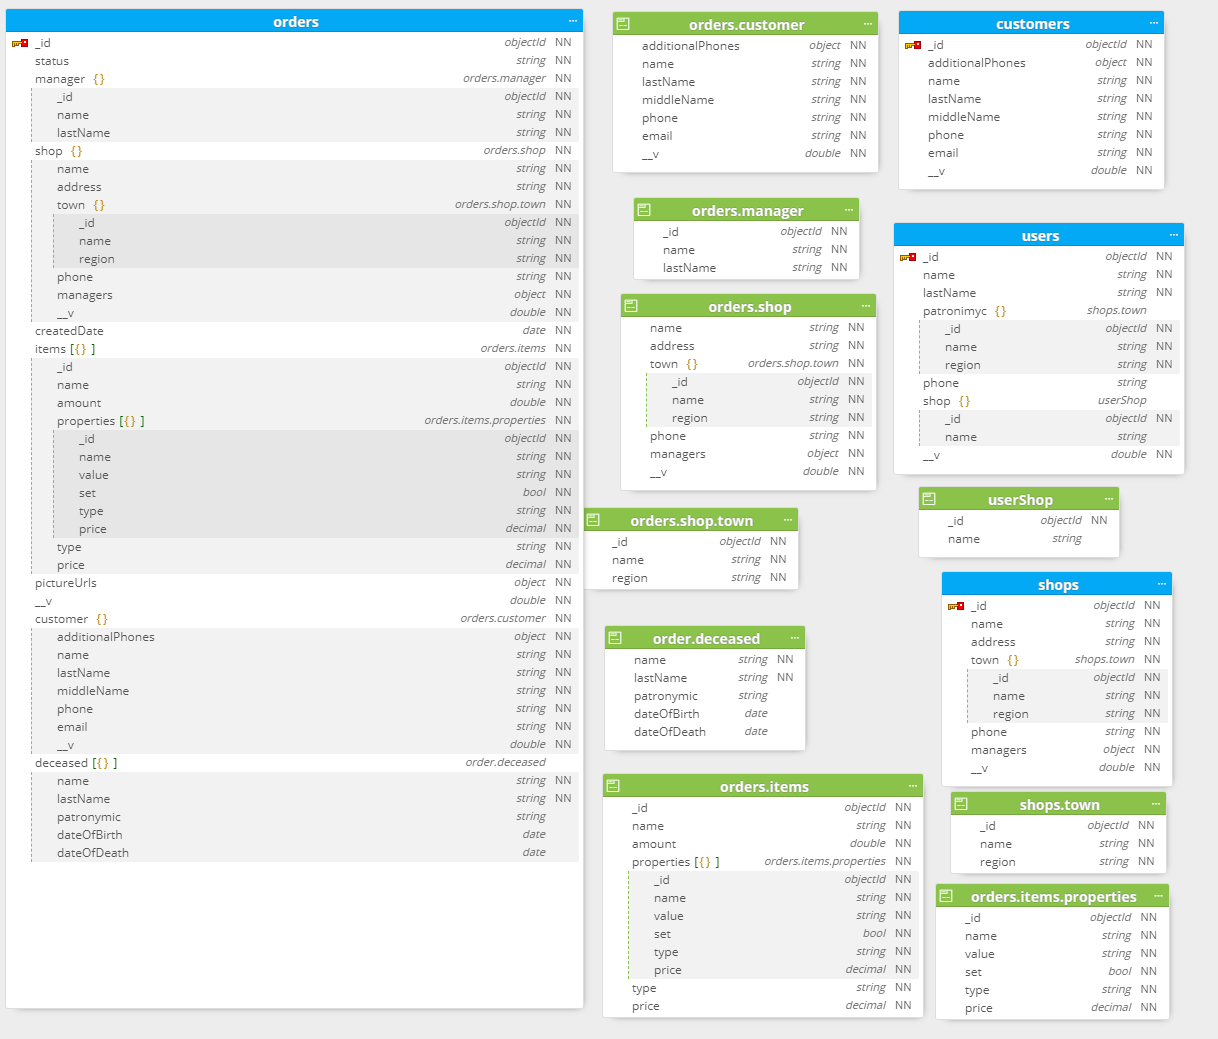
\includegraphics{images/dborder.png}}
\caption{\label{dborder} Диаграмма сущностей базы данных относящихся к функционалу создания заказа}
\end {center}
\end {figure}

\begin{figure}[ht]
\begin{center}
\scalebox{0.55}{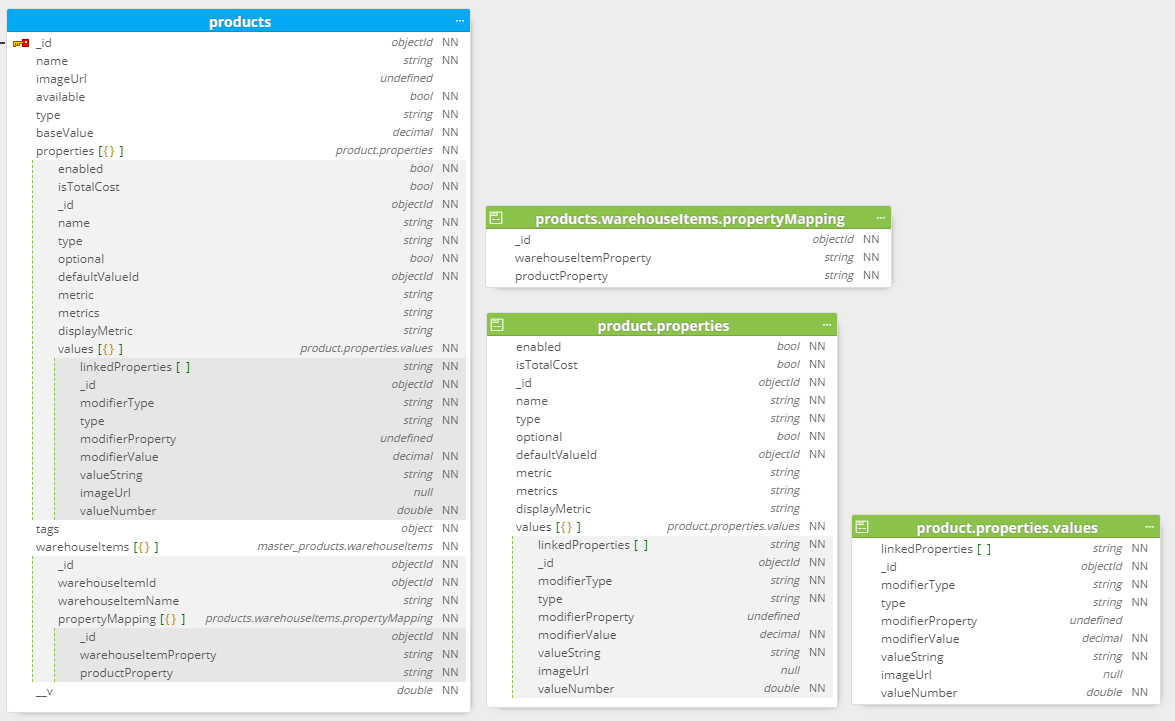
\includegraphics{images/db_products.png}}
\caption{\label{db_products} Диаграмма сущностей базы данных относящихся к функционалу каталога}
\end {center}
\end {figure}
\pagebreak

\subsection{Макет интерфейса}

Изначально макет интерфейса обсуждался напрямую с заказчиком, был сделан акцент на функционал форм,
 а также процесс добавления предметов в заказ и изменение состояния заказа.

Макет интерфейса программы разрабатывался в приложении Figma. Был разработан типовой дизайн компонентов интерфейса, 
а также несколько основных страниц как на настольном браузере, так и в мобильной версии.

Пример одной страницы представлен на рисунке \ref{mockup}.

\begin{figure}[ht]
\begin{center}
\scalebox{0.3}{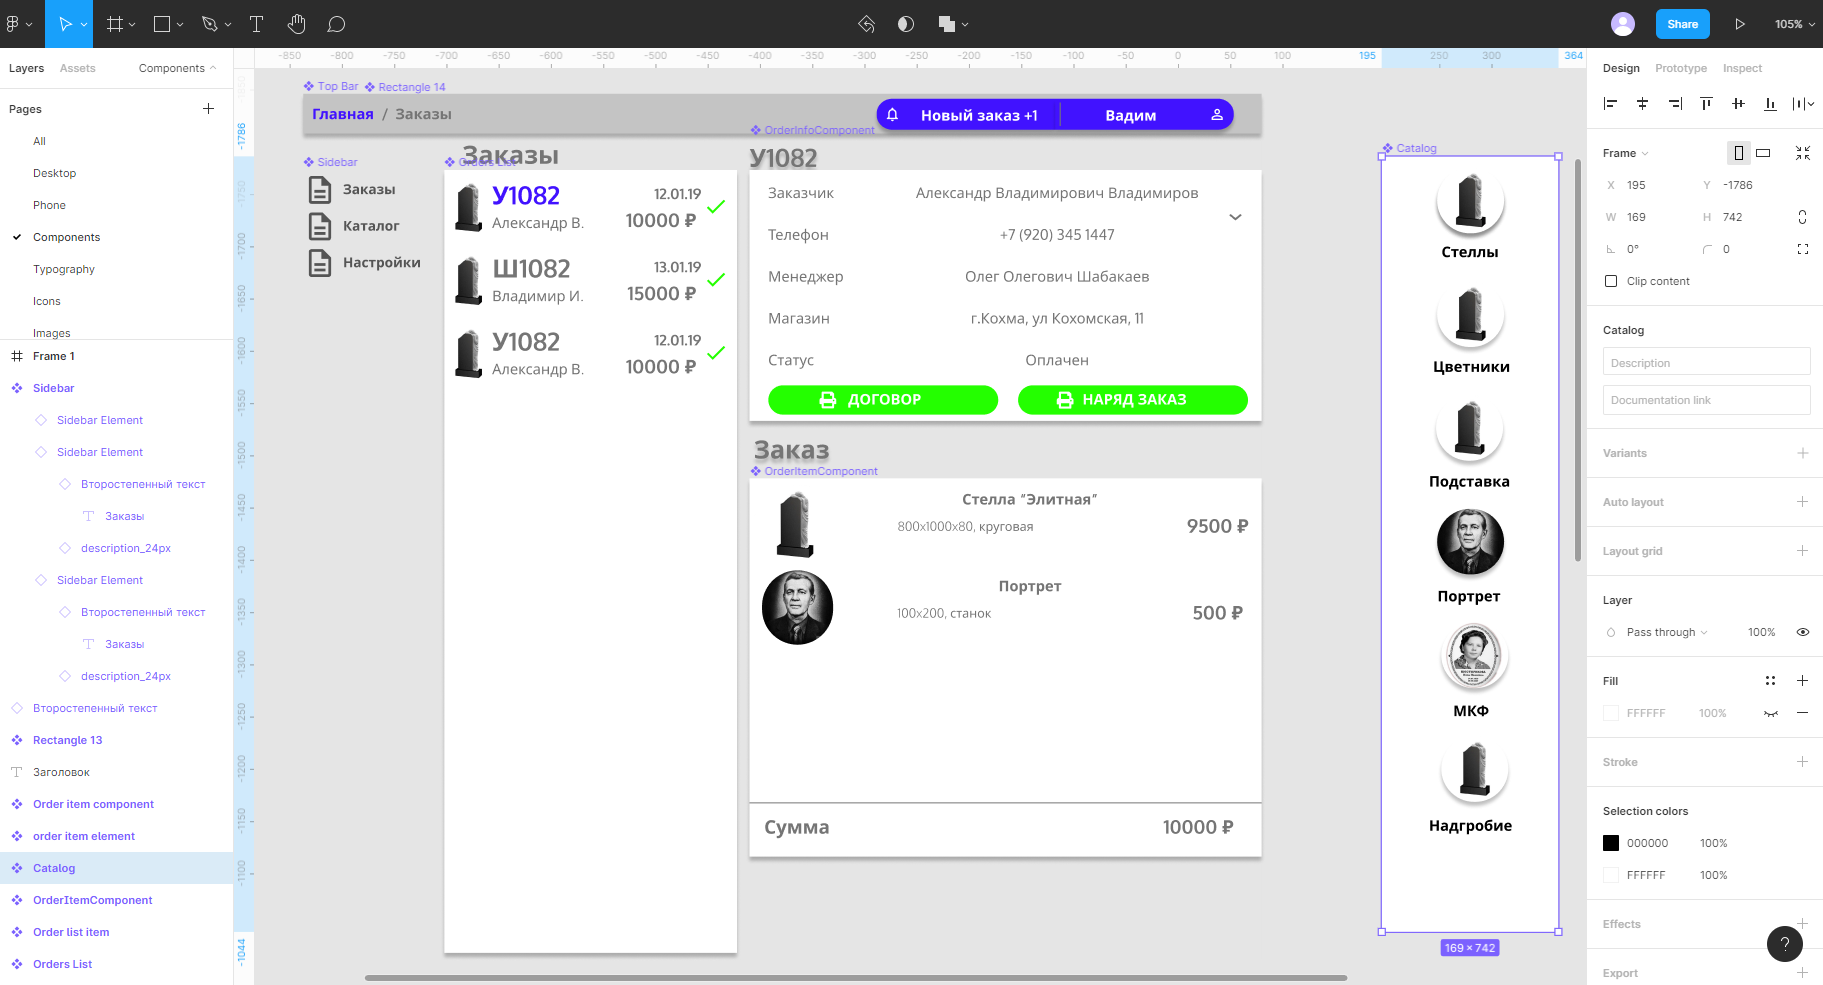
\includegraphics{images/mockup.png}}
\caption{\label{mockup} Пример макета одной из страниц приложения.}
\end {center}
\end {figure}

\section{Разработка}

\subsection{Разработка собственного набора компонентов}
\subsubsection{Обоснование}

Так как разработка проекта выполняется в рамках выпускной квалификационной работы, было решено создать свой набор компонентов,
с целью исследования возможностей библиотеки ReactJS а также получения новых навыков.

При использовании одной сторонней библиотеки возникает проблема ограниченности выбора компонентов.
При использовании нескольких сторонних библиотек компонентов возникает проблема их несовместимости и более того они выглядят некрасиво.

Такой библиотека поможет сделать приложение более консистентным

\subsubsection{Разработка}

Для разработки использовался фреймвок styled-components.

Который позволяет создавать стилизованные react компоненты с помощью backticks.
Это библиотека использует JSS, при этом используется синтаксис похожий на CSS [2].

В процессе разработки было решено, что для экономии времени и ресурсов, все компоненты будут в одном пакете,
который будет содержать как низкоуровневые стилизованные компоненты, так и высокоуровневые компоненты с
вспомогательной логикой.

В идеальном мире, нужно было разбить это на два разных пакета и сделать их независимыми, но 
было решено сделать переход к этой архитектуре постепенным.

\subsubsection{Результат}

Библиотека компонентов опубликована со свободной лицензией в публичный NPM registry с именем @dmitriiqq/react-kit.
\pagebreak

\section{Разработка мобильного приложения}

В рамках курса по разработки мобильных приложений был создан Proof-of-Concept мобильный клиент 
для системы на платформе ReactNative.

Данный клиент был предназначен для пользователей с ролью администратора, для того
чтобы быть всегда в курсе изменений происходящих в системе.

Например иметь всю информацию о заказах, также был реализован функционал редактирования каталога.

\subsection{Цели и задачи разработки приложения}

Приложение должно выполнять вспомогательные функции для управления системой,
чтобы облегчить ее администрирование, когда нет под рукой компьютера.

\subsection{Портрет целевой аудитории}
Целевой аудиторией являются пользователи системы для заказа памятников, 
управляющие бизнесом индивидуальные предприниматели, малый бизнес. Они работают 24/7,
всегда нужно решать какие то вопросы, даже когда под рукой нет компьютера.

\subsection{Краткое описание мобильного приложения}
Приложение позволяет администраторам системы достигать целей по управлению
системой заказа памятников: управлять персоналом, магазинами и каталогом изделий.

Варианты использования представлены в нотации UML на диаграмме \ref{mobileuml}.

\begin{figure}[ht]
\begin{center}
\scalebox{0.4}{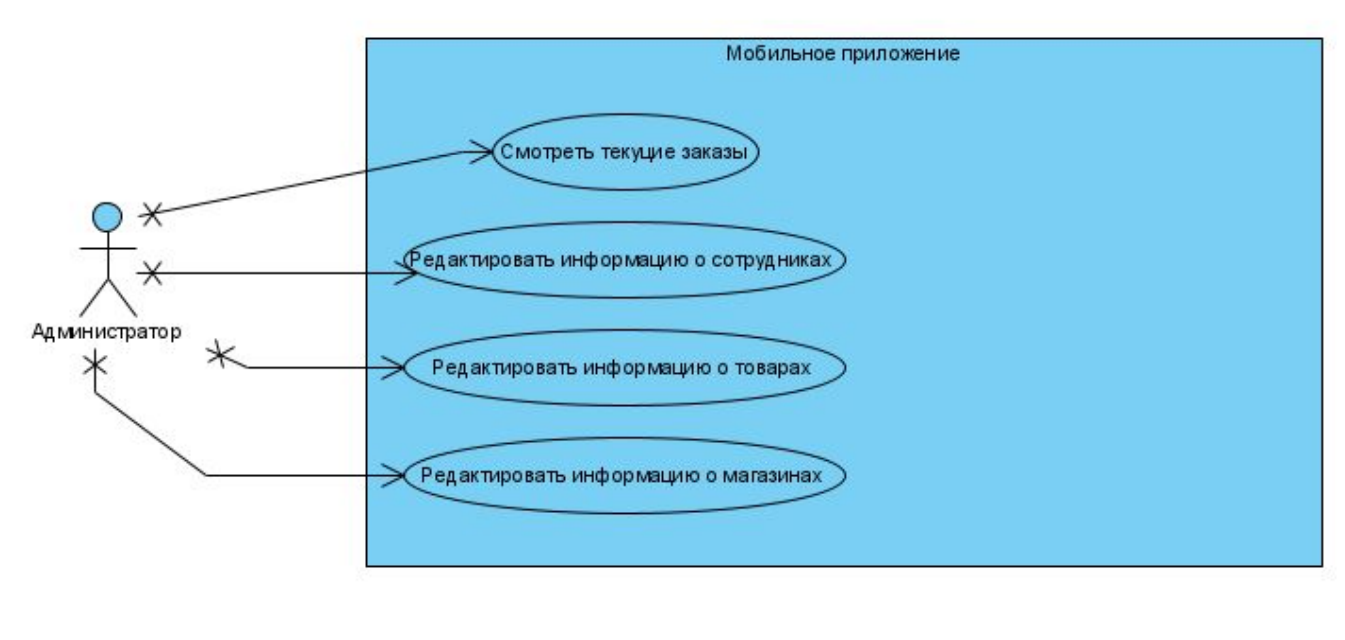
\includegraphics{images/mobileuml1.png}}
\caption{\label{mobileuml} Диаграмма сборки проекта}
\end {center}
\end {figure}

\subsection{Результат разработки}

Для разработки я использовал платформу ReactNative, так как она позволяет использовать
уже существующий код написанный для веб-клиента для бизнес логики программы и общения с API.

Единственное что нужно добавить - это слой представления. Он был реализован с помощью набора готовых компонентов
react-ui-kitten. Основные экраны приложения показаны на рисунке \ref{mobile}.

\begin{figure}[ht]
\begin{center}
\scalebox{0.3}{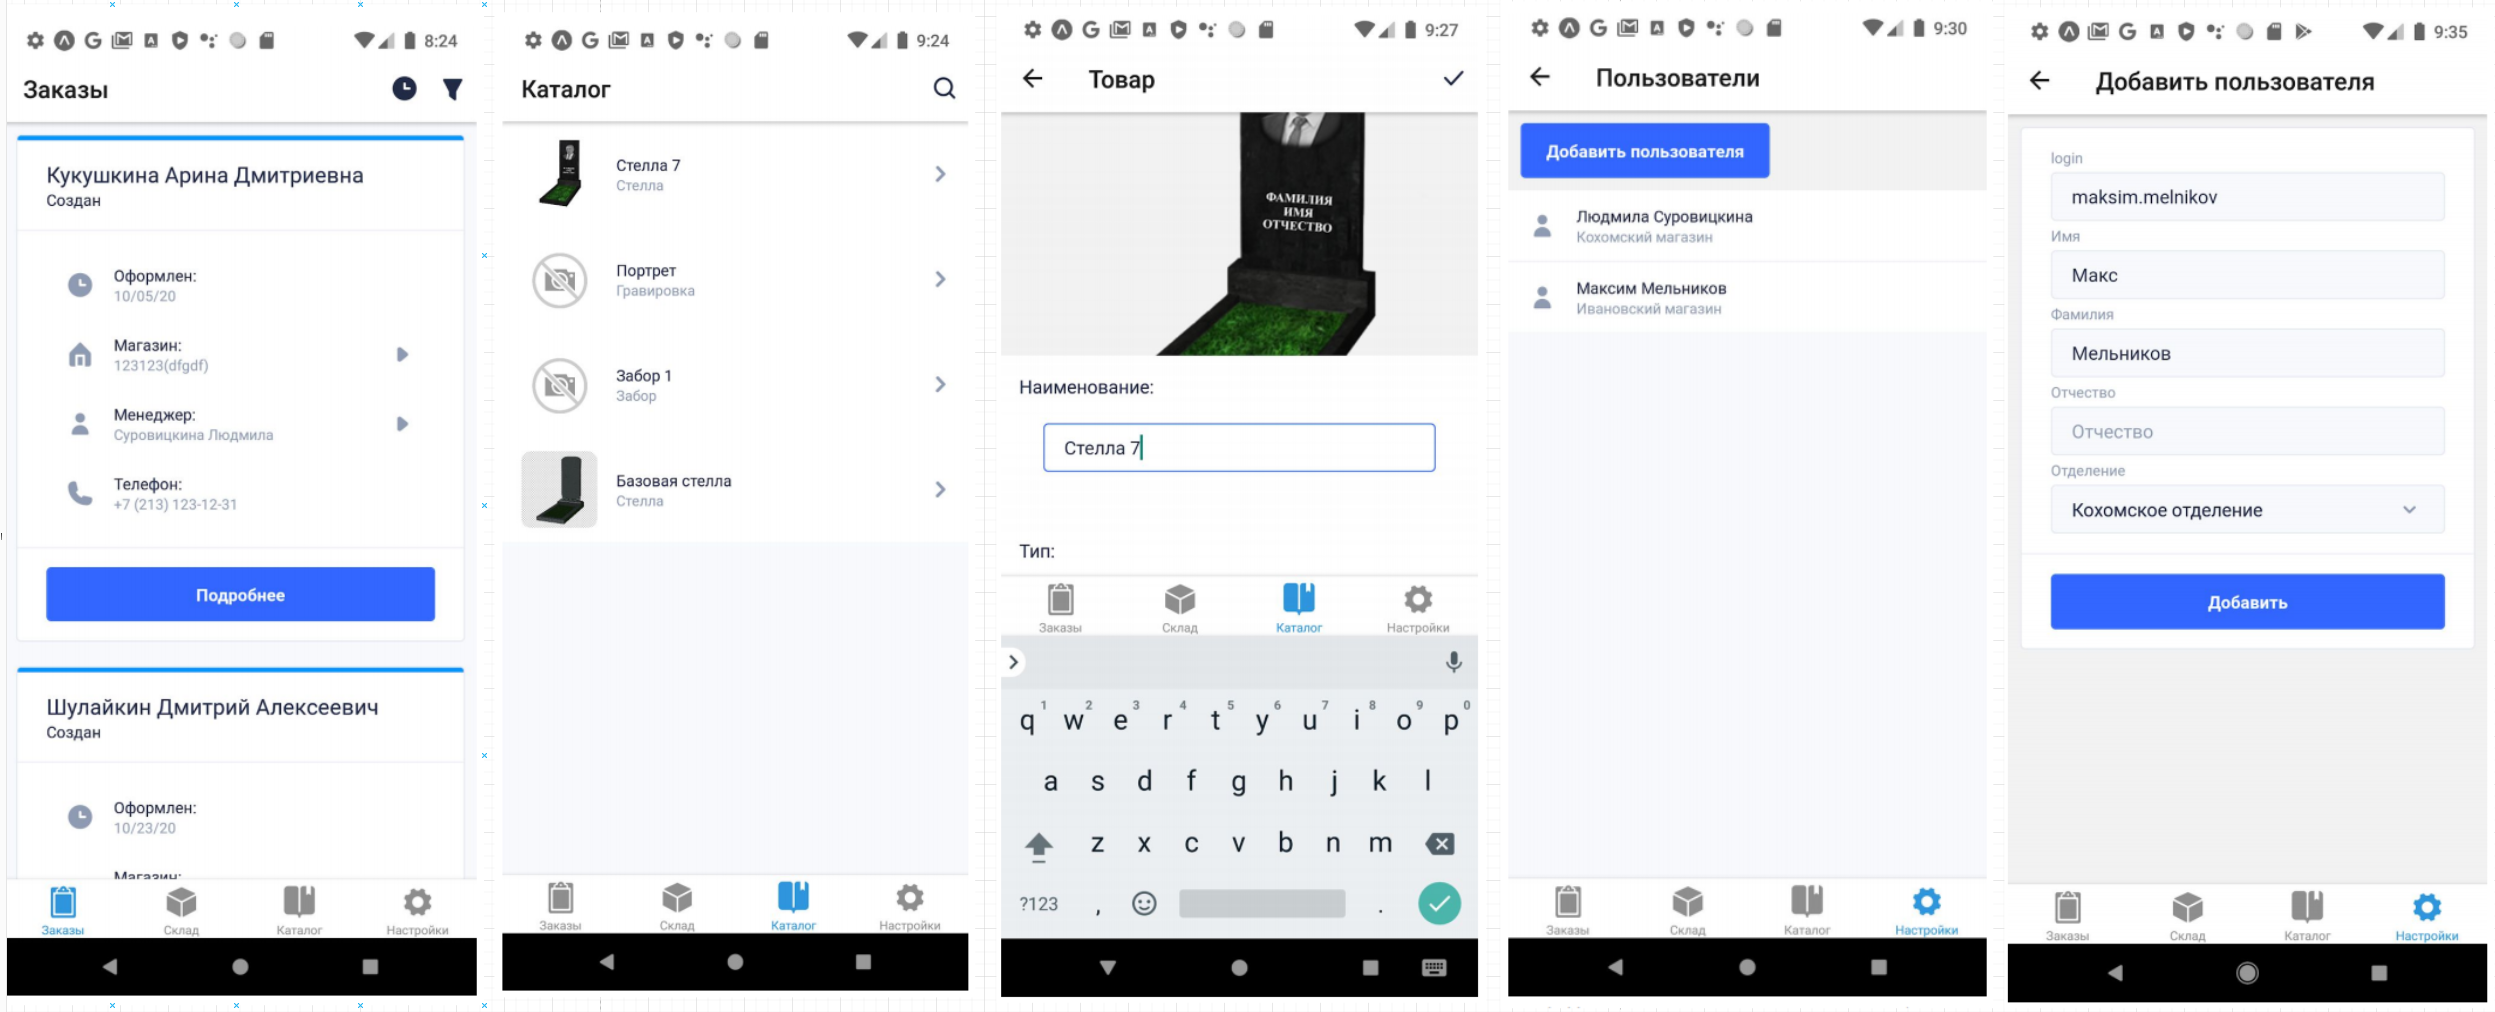
\includegraphics{images/mobile.png}}
\caption{\label{mobile} экраны приложения}
\end {center}
\end {figure}
\pagebreak

\section{Тестирование}
В данной главе описываются методы которые были применены при  тестировании приложения:

\begin{enumerate}
    \item Тестирование методом черного ящика
    \item Тестирование методом белого ящика
    \item Интеграционное тестирование
\end{enumerate}

\subsection{Тестирование методом черного ящика}

При тестировании методом черного ящика тестирующая система ничего не знает об исходном коде тестируемой системы.
Для тестирования методом черного ящика рассмотрим форму добавления информации о заказчике. 

Эта форма удовлетворяет вариант использования «Редактировать информацию о
заказчике». Интерфейс формы показан на рисунке \ref{tpo1}.

Определим классы эквивалентности:

\begin{enumerate}
    \item Телефон должен быть в формате +7 (999) 99-99-99. То есть начинаться с +7, вместо 9
    могут быть любые другие цифры от 0 до 9.
    \item email должен быть в формате example@email.com. Где example, email, com могут быть
    любыми строками содержащими только символы латинского алфавита, цифры и спец символы
    \item Фамилия, имя, отчество могут содержать только символы русского алфавита
    \item Фамилия, имя, отчество начинаются с большой буквы
    \item Телефон, фамилия, имя являются обязательными полями
\end{enumerate}

Так как выходным данным метода валидации является true/false у нас есть всего
два класса эквивалентности: допустимый класс и недопустимый класс
Для составления классов эквивалентности по спецификации можно рассмотреть
следующие ситуации относящиеся к допустимому классу:

\begin{enumerate}
    \item Все поля формы заполнены и содержат допустимые значения;
    \item Заполнены только минимально необходимые поля («телефон», «фамилия», «имя»), и
    эти поля содержат допустимые значения;
    \item Заполнены только минимально необходимые поля и поле «email», и эти поля содержат
    допустимые значения;
    \item Заполнены только минимально необходимые поля и поле «отчество», и эти поля
    содержат допустимые значения.
\end{enumerate}

Все остальные ситуации относятся к недопустимому классу:
\begin{enumerate}
    \item Одно или несколько обязательных полей не заполнены
    \item Одно или несколько из заполненных полей содержат недопустимые значения
\end{enumerate}


\begin{figure}[ht]
\begin{center}
\scalebox{0.4}{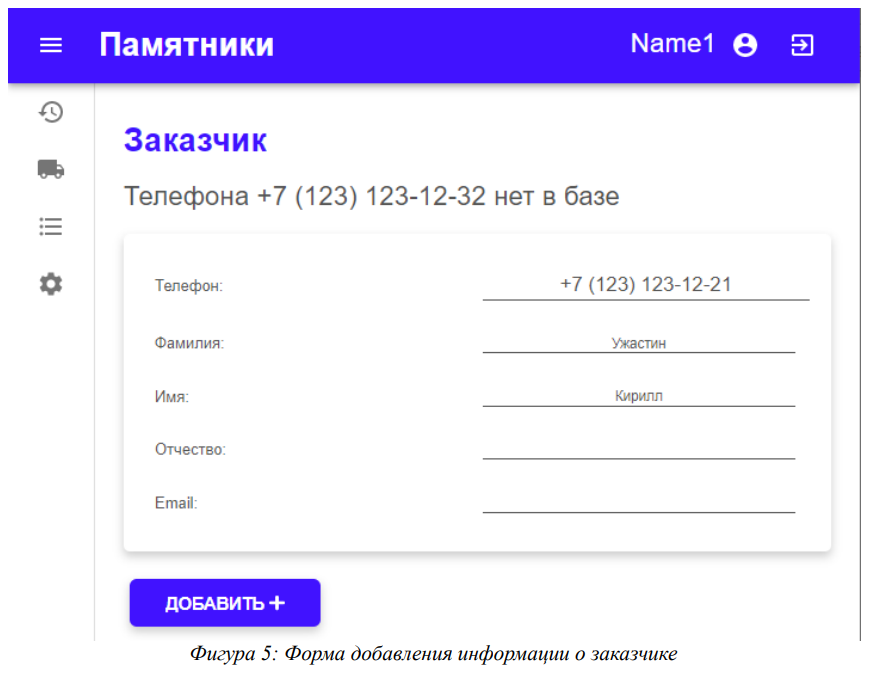
\includegraphics{images/tpo1.png}}
\caption{\label{tpo1} Диаграмма сборки проекта.}
\end {center}
\end {figure}

Для реализации unit-тестирования
используется тестовый фреймворк jest. Форма добавления информации о клиенте использует
метод validateCustomer который возвращает true или false. 

Согласно методу черного ящика
тестировщик не знает как устроен этот метод, а только что этот метод принимает в качестве
входных параметров и отдает на выход. При написании тестов тестировщик полагается
только на классы эквивалентности. Классы эквивалентности показаны в таблице \ref{tpo1table}. 

\begin{figure}[ht]
\begin{center}
\scalebox{0.7}{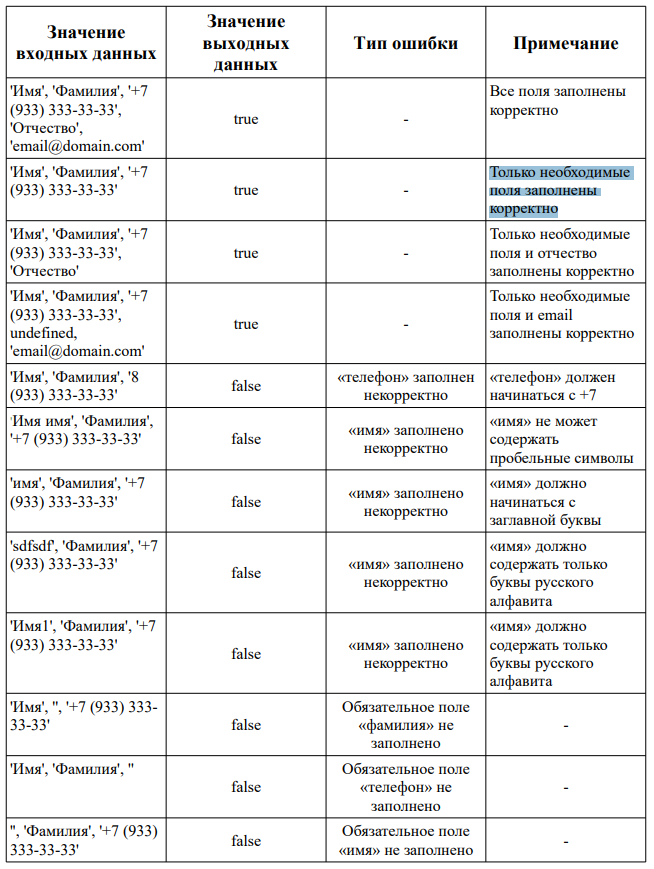
\includegraphics{images/tpo1table.png}}
\caption{\label{tpo1table} классы эквивалентности}
\end {center}
\end {figure}

\subsection{Тестирование методом белого ящика}

В качестве метода для демонстрации тестирования был выбран метод getPropertyCost, который используется в варианте использования 
``Добавить товар в заказ''. Этот метод вычисляет стоимость отдельного свойства памятника, например размер
или толщина.
Интерфейс формы добавит в заказ показан на рисунке \ref{tpo2}.

\begin{figure}[ht]
\begin{center}
\scalebox{0.7}{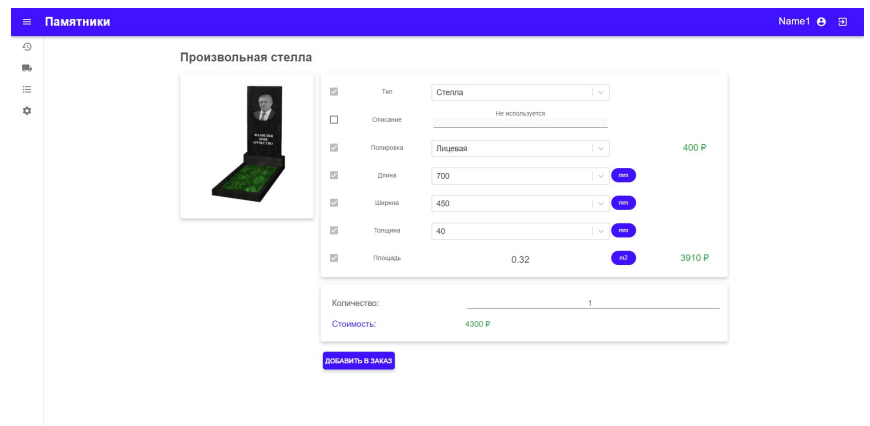
\includegraphics{images/tpo2.png}}
\caption{\label{tpo2} форма вычисления стоимости}
\end {center}
\end {figure}

Программа получает на вход описание свойства property, значение для которого
нужно вычислить стоимость, и уже вычисленные на данный момент свойства.

Так как стоимость одного свойства может зависеть от другого свойства, как
например стоимость полировки памятника может зависеть от площади памятника.
При вызове функции гарантируется что все зависимости свойства уже вычислены
и находятся в массиве computedProperties.

\begin{verbatim}
export const getPropertyCost = (
  property: MasterProductProperty,
  value: MasterProductPropertyValue,
  computedProperties: PropertyResponse[] = []
  ): number => { // 1


  if (!value) { // 2
    throw new ValidationError("No value provided"); // 3
  }

  const { modType, modifierValue } = value; // 4
  const modifierValueFloat = Number(modifierValue.toString());

  if (modType === ModifierType.Constant) { // 5
    return modifierValueFloat; //9
  } else if (modType === ModifierType.CostFromValue) { // 6
    if (!value.valueNumber) { // 10
      throw // 12
        new ConfigurationError(`...expected number property`) 
    }
    return modifierValueFloat * value.valueNumber; // 11
  } else if (modType === ModifierType.ProcentToPropertyCost) { // 7
    const modifierProperty = computedProperties
      .find(p => p.propertyName === value.modifierProperty);
    if (!modifierProperty) { // 13
      throw new Error("Failed to link..."); // 15
    }
      return value.modifierValue * modifierProperty.cost / 100; // 14
  } else if (modType === ModifierType.MultiplyPropertyCost) { // 8
    const modifierProperty = computedProperties
    .find(p => p.propertyName === value.modifierProperty);
    const modValueFloat = Number(value.modifierValue.toString()) || 1;
    if (!modProperty) { // 16
      throw new Error("Failed to link..."); // 19
    }
    if (!value.valueNumber) { // 17
      throw new Error("Failed to get valueNumber"); // 20
    }
    return value.valueNumber 
      * modalueFloat 
      * Number(modifierProperty.cost); // 18
  }
    
    return 0; // 21
} 
\end{verbatim}

Диаграмма УГП представлена на рисунке \ref{tpo2ugp}

\begin{figure}[ht]
\begin{center}
\scalebox{0.5}{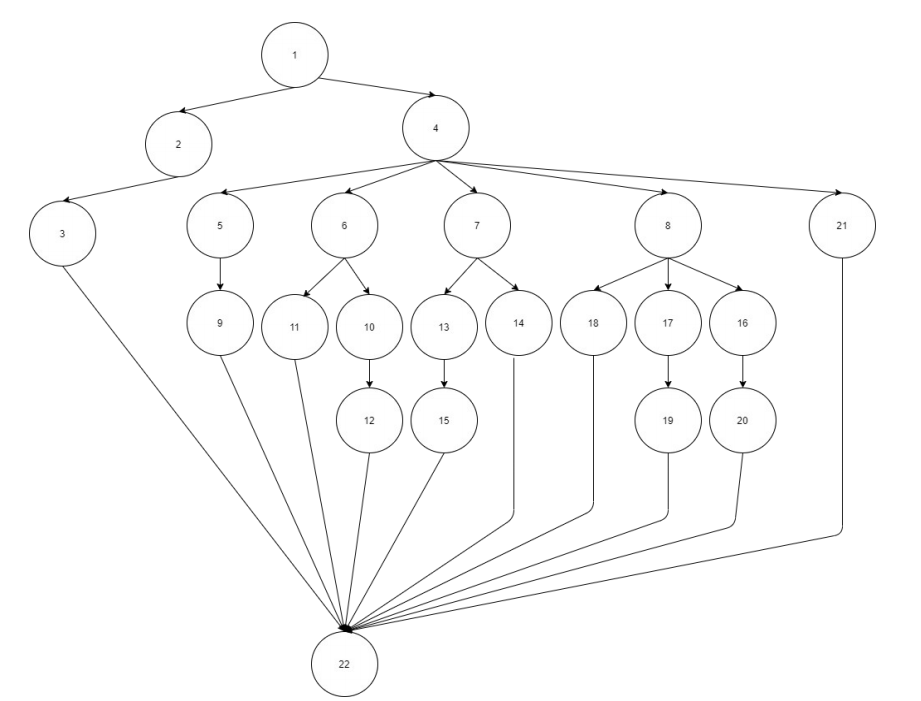
\includegraphics{images/tpo2ugp.png}}
\caption{\label{tpo2ugp} Диаграмма управляющего графа программы}
\end {center}
\end {figure}

Далее вычисляется цикломатическая сложность:

$$ V(G) = 30 \text{ дуг} - 22 \text{ узла} + 2 = 10 $$

Далее строится базовое множество независимых линейных путей

\begin{enumerate}
    \item 1,2,3,22
    \item 1,4,5,9,22
    \item 1,4,6,11,22
    \item 1,4,6,10,12,22
    \item 1,4,7,13,15,22
    \item 1,4,7,14,22
    \item 1,4,8,18,22
    \item 1,4,8,17,19,22
    \item 1,4,8,16,20,22
    \item 1,4,21,22
\end{enumerate}


\subsection{Интеграционное тестирование}

Для демонстрации интеграционного тестирования возьмем функционал создания записи
клиента. Будем тестировать серверную часть, а именно общение сервера и базы данных.

Так как в тесте участвуют сразу два компонента, сервер и база данных, такое тестирование
называют интеграционным.
Воспользуемся тестовым фреймворком jest. В качестве метода для тестирования
используем метод createCustomer.

\begin{verbatim}
  export const createCustomer = async (
  _: any,
  params: MutationCreateCustomerArgs
): Promise<Customer> => {
  const {
    name,
    lastName,
    middleName,
    phone,
    email,
    additionalPhones,
  } = params.input;

  if (!validateCustomer(params.input)) {
    throw new Error("Customer validation failed");
  }

  const document = await customerModel.create({
    name,
    lastName,
    middleName,
    phone,
    email,
    additionalPhones,
  });

  return getCustomerView(document);
};
\end{verbatim}

Этот метод общается с базой данных, он использует модель сущности Mongoose,
для интеграционного тестирования нам потребуется развернуть базу данных mongo.

\begin{verbatim}
  import {
    customerByPhone,
    createCustomer,
  } from "../resolvers/CustomersResolver";
  
  const dbHandler = require("./inMemoryDB");
  
  const getCustomer = (
    name: string,
    lastName: string,
    phone: string,
    middleName?: string,
    email?: string
  ) => ({
    name,
    middleName,
    lastName,
    phone,
    email,
    additionalPhones: [],
  });
  
  beforeAll(async () => await dbHandler.connect());
  
  afterEach(async () => await dbHandler.clearDatabase());
  
  afterAll(async () => await dbHandler.closeDatabase());
  
  describe("customer ", () => {
    it("can be created correctly", async () => {
      const createCustomerParams = getCustomer(
        "Имя",
        "Фамилия",
        "+7 (933) 333-33-33",
        "Отчество",
        "email@domain.com"
      );
  
      const customer = await createCustomer(null, {
        input: createCustomerParams,
      });
  
      expect(customer!.id).toBeDefined();
      expect(customer!.name).toBe("Имя");
      expect(customer!.lastName).toBe("Фамилия");
      expect(customer!.middleName).toBe("Отчество");
      expect(customer!.phone).toBe("+7 (933) 333-33-33");
      expect(customer!.email).toBe("email@domain.com");
  
      const newCustomer = await customerByPhone(null, {
        phone: "+7 (933) 333-33-33",
      });
  
      expect(newCustomer!.id).toBe(customer.id);
      expect(newCustomer!.name).toBe("Имя");
      expect(newCustomer!.lastName).toBe("Фамилия");
      expect(newCustomer!.middleName).toBe("Отчество");
      expect(newCustomer!.phone).toBe("+7 (933) 333-33-33");
      expect(newCustomer!.email).toBe("email@domain.com");
    });
  
    it("validates user phone", async () => {
      await expect(async () => {
        const createCustomerParams = getCustomer(
          "Имя",
          "Фамилия",
          "8 (933) 333-33-33"
        );
        await createCustomer(null, { input: createCustomerParams });
        return true;
      }).rejects.toThrow();
    });
  });
  
\end{verbatim}

Данная проблема решается с помощью пакета mongodb-memory-server, который позволяет запустить базу
данных mongo внутри оперативной памяти компьютера только на время тестов. Логика
запуска базы данных общая для всех тестов и находится в файле inMemoryDB.js.

\begin{verbatim}
  const mongoose = require('mongoose');
  const { MongoMemoryServer } = require('mongodb-memory-server');
  
  const mongod = new MongoMemoryServer();
  
  module.exports.connect = async () => {
      const uri = await mongod.getUri();
  
      const mongooseOpts = {
          useNewUrlParser: true,
          autoReconnect: true,
          reconnectTries: Number.MAX_VALUE,
          reconnectInterval: 1000
      };
  
      await mongoose.connect(uri, mongooseOpts);
  };
  
  module.exports.closeDatabase = async () => {
      await mongoose.connection.dropDatabase();
      await mongoose.connection.close();
      await mongod.stop();
  };
  
  module.exports.clearDatabase = async () => {
      const collections = mongoose.connection.collections;
  
      for (const key in collections) {
          const collection = collections[key];
          await collection.deleteMany();
      }
  };
\end{verbatim}


\section{Сборка проекта}

Итогом сборки проекта должен стать один Docker image, в котором должны быть упакованы файлы полученные при сборке 
пакетов web и api. В качестве базового образа используется обычный образ node:14. 

Перед тем, как начать финальную сборку, нужно убедиться что пакеты core, graphql были опубликованы в NPM registry.
Так как эти пакеты должны будут потом установиться внутрь Docker image при установке зависимостей api.

Сборка docker image проходит в два этапа:

\begin{enumerate}
    \item Сначала создается временный контейнер в который копируются весь код из репозитория нужный для сборки,
    потом выполняются все скрипты build во всех проектах моно-репозитория. 
    \item Полученные артефакты сборки web и api копируются в финальный образ 
    докера. Внутри финального образа устанавливаются зависимости api.
\end{enumerate}

Полученный Docker образ нужно в дальнейшем загрузить в docker registry.
Полная диаграмма сборки показана на рисунке \ref{build}.

\begin{figure}[ht]
\begin{center}
\scalebox{0.4}{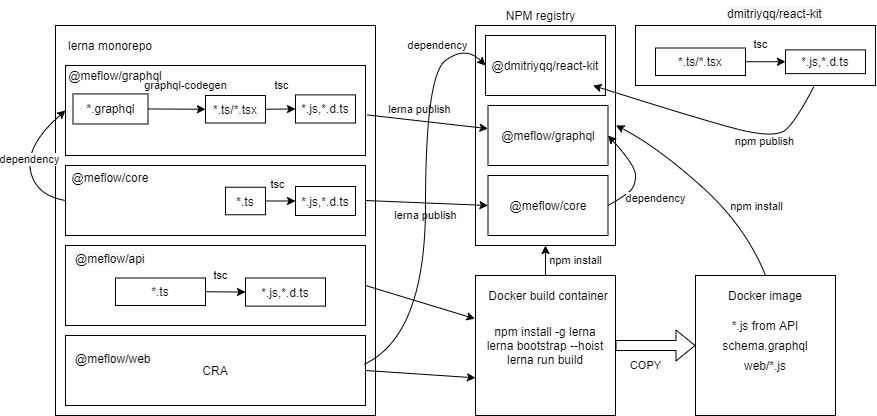
\includegraphics{images/build.png}}
\caption{\label{build} Диаграмма сборки проекта.}
\end {center}
\end {figure}

\section{Разворачивание приложения}

Самый простой, универсальный и популярный способ развернуть docker приложение это k8s.
Для самого приложения я использую простой deployment, так как мое приложение не использует состояния.

Кроме самого приложения также разворачивается сервис ClusterIP который выполняет роль LoadBalancer внутри кластера,
а также nginx-ingress который позволяет обрабатывать внешние запросы. 
Также в kubernetes должен быть Issuer сертификатов чтобы поддерживать протокол TLS.

Полная диаграмма k8s показана на рисунке \ref{k8s}

\begin{figure}[ht]
\begin{center}
\scalebox{0.4}{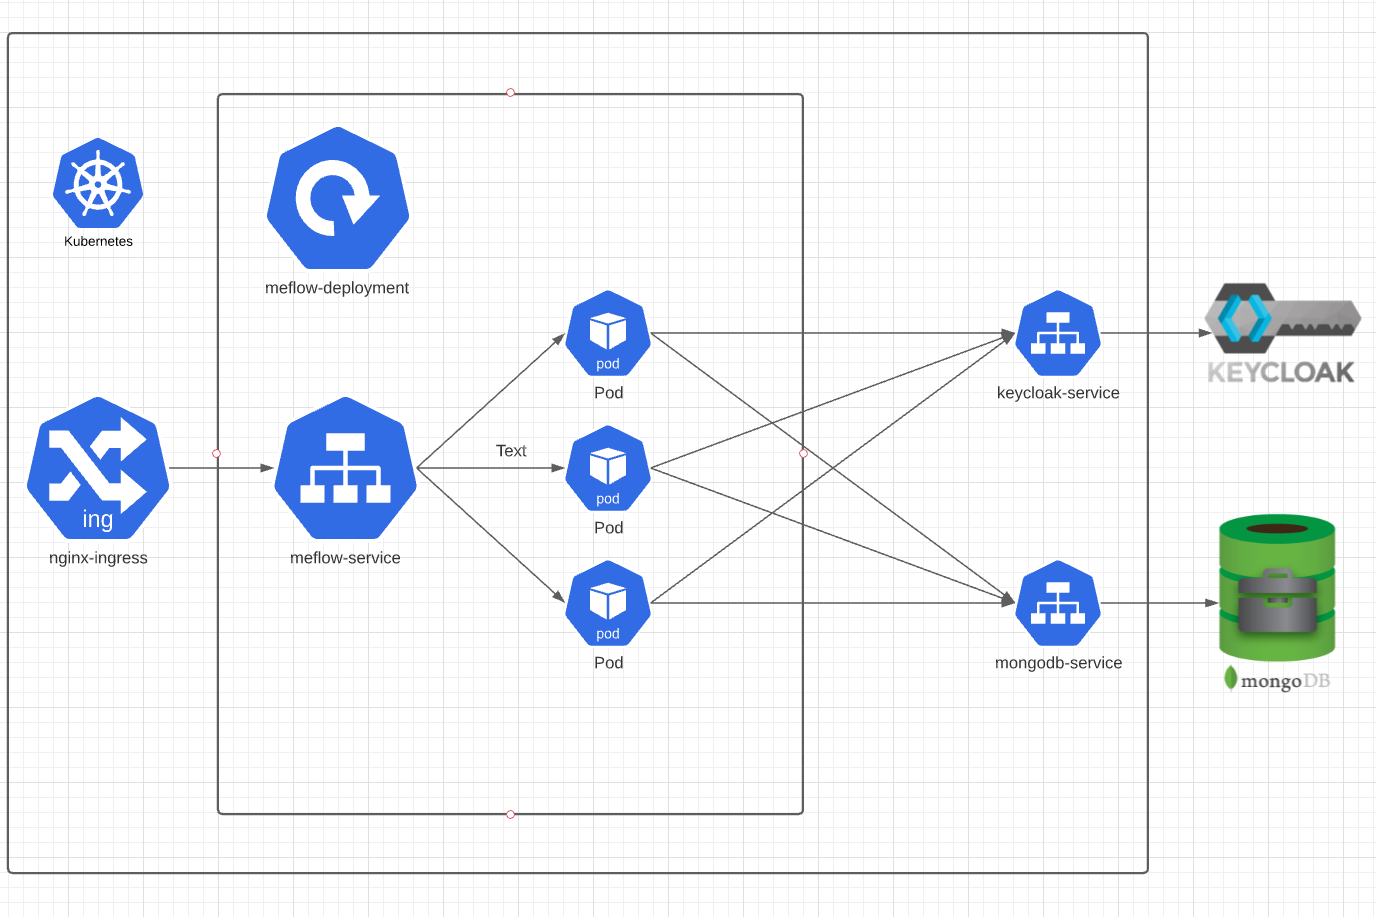
\includegraphics{images/deploy.png}}
\caption{\label{k8s} Диаграмма разворачивания проекта.}
\end {center}
\end {figure}


\specialsection{Заключение}

Целью данной работы являлась разработка веб-приложения для заказа памятников.

Была проведена работа по анализу требований, проектированию и разработке веб-приложения для заказа памятников.
Организовано тестирование и развертывание приложение.

Разработан универсальная библиотека компонентов ReactJS используемая в веб приложении.

А также были созданы POC интернет-магазина и приложения для мобильных телефонов на базе Android и iOS способное взаимодействовать с системой,
как альтернативный клиент для некоторых вариантов использования.

В результате было получено готовое приложение которое решает проблемы и удовлетворяет потребностям заказчика.
\pagebreak

% Библиография в cpsconf стиле
% Аргумент {1} ниже включает переопределенный стиль с выравниванием слева
\begin{thebibliography}{1}
    \bibitem{voc} Introduction to Apollo Server [Электронный ресурс]. Режим доступа: https://www.apollographql.com/docs/apollo-server/. – Заглавие с экрана. – (Дата обращения 13.06.2021)
    \bibitem{vo2} Styled Components Documentation [Электронный ресурс]. Режим доступа: https://styled-components.com/docs. – Заглавие с экрана. – (Дата обращения 13.06.2021)
\end{thebibliography}
\end{document}
\pagebreak

\specialsection{Приложение А}

\specialsection{Приложение B}

\pagebreak

